From a macroscopic perspective, nuclei can be viewed as charged particles, and thus collisions (here in a loose sense) between them are governed by the Rutherford scattering formula.
This is how the nucleus was discovered in the first place. However, this simple picture breaks down at higher energies, when the particles are able to cross the Coulomb barrier.
At yet higher energies, when the de Broglie wave-length ($\lambda \sim \vec{p}^{-1}$) becomes sufficiently small to resolve the inner structure of the nuclei, it becomes feasible to model the collision as not taking place between the two nuclei, but by individual protons and neutrons (nucleons).

This leads us to the \emph{participant-spectator} picture of nuclear collisions, in which the collision is viewed as if taking place between a few \emph{participant} nucleons, while the remaining \emph{spectator} nucleons remain mostly unaffected. Such a reaction is known as \emph{quasi-elastic scattering}, since the kinetic energy of the projectile is much greater than the binding energy of the participants, which further motivates treating them as approximately free particles. This also means that the kinetic energy will almost be conserved, hence \emph{quasi-elastic}.
The collision between the participant nucleons takes place at a time scale of about \unit[$10^{-23}$]{s}\cite{gaimard:1991:art}, and is sometimes called a \emph{fireball} or \emph{firestreak}.

However, this is just the first part of the collision. The spectator nucleons may have gone unaffected through it, but the resulting system (a so-called pre-fragment) will be highly excited, and will decay to the final fragment -- often by ejecting nucleons, in this context known as evaporating them. The characteristic time-scale for these ejections varies between \unit[$10^{-21}$ -- $10^{-16}$]{s}, depending on the energies and emitted particle\cite{gaimard:1991:art}. 

In this picture, a two-step process can be used to describe nuclear fragmentation. 
Various models to describe both steps exist in the literature, and these can be combined more or less freely -- restrictions arise since they do not necesarilly use the same parameters. Models which mainly use parameters like $A$, the number of nucleons, $Z$ the number of protons, the total nuclear-spin $J$ and the excitation energy $E$ of the nucleus are termed \emph{macroscopic}, while models that directly treat the states of individual nucleons are called \emph{microscopic}. Examples of the former are the \emph{abrasion-ablation model}\cite{bowman:1973:book}, while the \emph{intranuclear-cascade model}\cite{metropolis:1991:art} is an example of a microscopic model. As it is often the case in nuclear physics, no one model is valid for the whole range of nucleon numbers $A$ and incident energies\cite{cucinotta:1998:art}.

Since the focus of this report is to describe an event-generator for a physics experiment, we can afford to use less detailed models if this reduces computation time. In addition, since the macroscopic properties of nuclei are more easily related to expermental observables, we will restrict our attention to those. 

\subsection{The fast processes -- the Goldhaber model}
\label{sec:fast}
%!!! SUDDENLY, CODE. INTRODUCE MODEL FIRST? !!!
%To mimic existing code !!!CITE LEONID?!!! and to allow the user to study a reaction of their interest, the outcome of the first stage of the process is largely determined by user input: the participant projectile nucleons -- the cluster -- as well as its invariant mass, and the excitation energy of the pre-fragment are both specified by user input. The only specific model used is to determine the momentum of the participant system relative to the projectile, everything else is just conservation of momentum, and an isotropic cross-section. 
%The \emph{Goldhaber model} states that the momentum distribution is given by a Guassian with the width determined by the expectation value of the momentum of an individual nucleon, explicitly
%\begin{equation}
%\sigma^2 = \langle \vec{p}^2 \rangle A\frac{A_\text{p}-A}{A_\text{p}-1},
%\end{equation}
%where $A_\text{p}$ is the number of nucleons in the projectile, $A$ in the pre-fragment, and $\langle \vec{p}^2 \rangle$ is the expectation value of the momentum of an individual nucleon. For a Fermi-gas, $\langle \vec{p}^2 \rangle$ may be written in terms of the Fermi-momentum $\vec{p}_f$ as $\tfrac{3}{5} \vec{p}_f^2$\cite{goldhaber:1974:art}.
In the participant-spectator picture, the fast process consists of a collision between the target and a cluster within the projectile nucleus. This is determined by momentum conservation, but in order to apply this, we need to know the initial momentum of the internal cluster, which will have a momentum relative to the projectile. The situation is illustrated in \autoref{fig:fast}. 

\begin{figure}
\centering
\input{figures/fast-theory/fast.pdf_t}
\caption{\label{fig:fast} The fast process. The projectile ($A$) is viewed as a system of a cluster and prefragment. The collision then takes place between the cluster and the target.}
\end{figure}

The \emph{Goldhaber model} states that the 3-momentum distribution is given by a Guassian with the width determined by the expectation value of the momentum of an individual nucleon, explicitly
\begin{equation}
\sigma^2 = \langle \vec{p}_\text{nucleons}^2 \rangle A'\frac{A_\text{C}}{A-1},
\end{equation}
where $A$ is the number of nucleons in the projectile, $A' = A-A_\text{cluster}$ the nucleon number of the prefragment, and $\langle \vec{p}_\text{nucleons}^2 \rangle$ is the expectation value of the 3-momentum of an individual nucleon. For a Fermi-gas, $\langle \vec{p}^2 \rangle$ may be written in terms of the Fermi-momentum $\vec{p}_f$ as $\tfrac{3}{5} \vec{p}_f^2$\cite{goldhaber:1974:art}.
The nuclear Fermi-momentum, assuming a constant density, is about $\unit[270]{MeV}$, which is in reasonable agreement with experiments for heavier ($A>40$), non-exotic nuclei\cite{moniz:1971}. 

However, \rtb{} experiments are not necesarilly about heavy (and non-exotic) nuclei. Another model -- also a ``Goldhaber model'', since it uses a Guassian momentum distribution -- gives $\sigma^2$ as
\begin{equation}
\sigma^2 = 2 (M_{A'} + M_\text{C} -M_A) \frac{M_\text{C}M_{A'}}{M_\text{C}+M_{A'}} = -2 Q \mu(M_\text{C},M_{A'}),
\end{equation}
where $M_\text{C}$ is the mass of the participant cluster, $M_A$ the mass of the projectile and $M_{A'}$ the mass of the prefragment. If we take $-Q=T = \mu v^2/2$, we get $\sigma^2 = \mu^2 v^2$, which is the initial squared momentum of the cluster, provided that we can neglect the kinetic energy of $A'$. This model is suitable for lighter particles, since it requires that $M_{A'} + M_\text{C} -M_A = -Q >0$, or $\sigma^2$ becomes negative. This is the model used in this work.

Momentum conservation implies that
\begin{align}
p_{A} &= p_\text{C} + q_{A'} \\
p_\text{C} + p_\text{T} &= q_\text{C} + q_\text{T}
\end{align}
where the momenta are defined in \autoref{fig:fast}, with the additional definition of $A'=A-A_\text{C}$.
%$p_\text{A}$ is the 4-momenum of the projectile, $p_\text{T}$ the momentum of the target, $p_\text{C}$ the internal momentum of the cluster; $q_\text{A'}$ the final momenum of the prefragment, $q_\text{C}$ and $q_\text{T}$ the final momentum of the target and cluster, respectively.
The initial momentum of the cluster, $p_\text{C}$, in addition to being partly defined by the Goldhaber model, is also fully specified by the external momenta: viewing \autoref{fig:fast} as a Feynman diagram even makes it clear that the cluster is \emph{off-shell}.
With this in mind, we solves the first of the above equation for $p_\text{C}$ by squaring, which gives
\begin{equation}
M_\text{C,off}^2 \equiv p_\text{C}^2 = p_\text{A}^2 +  q_\text{A'}^2 -  2p_\text{A}\cdot q_\text{A'} =M_\text{A}^2 + M_\text{A'}^2 - 2M_\text{A}\sqrt{M_\text{A'}^2 + \vec{p}_\text{C}^2},\label{eq:offmass}
\end{equation}
where we have evaluated $p_\text{A}\cdot q_\text{A'}$ in the rest-frame of the prefragment. Note that since the prefragment is excited $M_\text{A'}$ will have to be adjusted by adding the excitation energy.

Since we are interested in constructing an event generator, we next transform the 4-momentum of the cluster from the projectile to the laboratory frame (the projectile and target momentum are already known in the laboratory frame -- the former being zero is practically the definition of that frame). The relevant gamma factor is
$\gamma = 1 + T/M_A$, where $T$ is the kinetic energy of the projectile.

Since the collision between the target and the cluster is easier to do in their center-of-mass (CM) frame\footnote{Strictly speaking, their zero momentum frame, or center-of-momentum frame.}, we also need to transform between the laboratory and that frame. This is readily done by noting
\begin{equation}
\bar{\vec{P}} \equiv \vec{p}_\text{C} + \vec{p}_\text{T} = \gamma(\beta_\text{ZM}) \bar{m} \vec{\beta}_\text{CM} = \bar{E}\vec{\beta}_\text{CM} \implies \vec{\beta}_\text{CM} = (\vec{p}_\text{C} + \vec{p}_\text{T})/\bar{E},
\end{equation}
where the barred quantities are of the system of both particles. Since we want the $\beta$ between the laboratory and the CM frame, we evaluate all the quantities in the laboratory frame
\begin{equation}
\vec{\beta}_\text{CM} = \frac{\vec{p}_\text{C}}{E_\text{C} + M_\text{T}}. \label{eq:betazm}
\end{equation}

The scattering between target and cluster is back-to-back in the CM frame, and we generate the scattering angle from an isotropic $\tfrac{d\sigma}{dt}$, which in practice means that the Mandelstam variable $t=(p_\text{C}-q_\text{C})^2$ is a uniform random number. The CM energy, momentum and scattering angle can be readily expressed in terms of the invariant Mandelstam variables% $s=(p_\text{C}+p_\text{T})^2$
\begin{align}
E_\text{C} &= \frac{s+M_\text{C,off} - M_\text{T}}{2\sqrt{s}} \\
|\vec{p}_\text{C}| &= \sqrt{E_\text{C,initial}^2 - M_\text{C,off}^2} \\
|\vec{q}_\text{C}| &= \sqrt{E_\text{C,final}^2 - M_\text{C}^2} \approx |\vec{p}_\text{C}|\\
\cos{\theta} &\approx \frac{t-N_\text{C}^2-N_\text{C}^2 + 2E_\text{C}^2}{2|\vec{p}_\text{C}|^2},
\end{align}
the approximations being valid under the assumption of a quasi-elastic scattering, more explicitly when $M_\text{C,off} \approx M_\text{C}$, so that $\vec{p}_\text{C} = -\vec{q}_\text{C}$ in the CM frame, which is the assumption used in deriving the equation for $\cos{\theta}$. %Together with \eqref{eq:offmass}, this quanitifies the notition of a collision being excited enough to approximately conserve kinetic energy:
%\begin{equation}
%M_\text{C} \approx M_\text{C,off} \implies 
%\end{equation}

A random polar angle $\phi$ in $[0,2\pi]$ is then generated, which together with $|\vec{p}_\text{c}|$, $\theta$ and $E_\text{c}$ fixes the CM 4-momentum of the cluster, and also the target by $\vec{p}_\text{t} = -\vec{p}_\text{c}$. Using \eqref{eq:betazm}, these results are boosted to the lab frame, in which we now have an expression for all the relevant momenta.

\subsection{The slow process -- decay of a compound nucleus}
%There are at least two models for the decay of a compound nucleus popular in the literature, the Hauser-Feshbach and the Ewing-Weisskopf formulas. Both aim to describe how a compound nucleus in a given macro-state ($E*$, $J$, $Z$, $A$) will decay.
%To describe the decay of a compound nucleus in a given macro-state ($E*$, $J$, $Z$, $A$), we need the probabilities to go from this state to any other macro-state. Since the only way an isolated nuclei can lose energy, angular momentum, or nucleons is by emitting particles, it is natural to view the transition probability as in terms of quantities related to particle emission.
%Hence, we expect the transition probability to depend on the type of particle emitted, $\nu$, the kinetic energy of this particle, $\epsilon_\nu$, and the angular momentum carried away by it.
%We will restrict ourselves to the case where this transition probability only depends on the type of particle
%There are at least two models for the decay of a compound nucleus popular in the literature, the Hauser-Feshbach and the Ewing-Weisskopf formulas. Both aim to describe how a compound nucleus in a given macro-state ($E*$, $J$, $Z$, $A$) will decay.
To describe the decay of a compound nucleus in a given macro-state ($E^*$, $J$, $Z$, $A$), we need the probabilities to go from this state to any other macro-state. Since the only way an isolated nuclei can lose energy, angular momentum, or nucleons is by emitting particles, it is natural to view the transition probability as in terms of quantities related to particle emission.

The formula used to describe this gives the probability of decaying by evaporating a particle $\nu$ as
\begin{equation}
\frac{d^2 P_\nu}{dE_f^* dt} = \frac{1}{\hbar} \frac{\rho(E_f^*,J_f)}{\rho(E_i^*,J_i)} \sum_{S=|J_f-s|}^{|J_f+s|}\sum_{l=|J_i-S|}^{|J_i+S|} T_l(\epsilon_\nu),\qquad\cite{schmidt:1991:art}\label{eq:ew}
\end{equation}
where $P$ is the probability, $E_f^*$ the final-state excitation energy, $J_f$ the final-state spin, $\rho$ the level densities and 
\begin{equation}
\epsilon_\nu \approx E_f^*-E_i^*-S_\nu\label{eq:kine}
\end{equation}
the kinetic energy of the evaporated particle, $S_\nu$ being its separation energy $S_\nu = M_f + m_\nu - M_i$\footnote{The approximation is due to neglecting the kinetic energy of the daughter nucleus, which should be a good approximation when the evaporated particle $\nu$ is light. This is not a necesary approximation, though, and a more exact formula is $\tfrac{m_\nu}{\mu}\epsilon_\nu \approx E_f^*-E_i^*-S_\nu$. The separation energy does not enter as a cost of removing the particle $\nu$, but rather to relate the two excitation energies $E_f^*$ and $E_i^*$ to an absolute scale.}. 
 Continueing: $s$ is the intrinsic spin of the evaporated particle, $S$ is the spin of the system consisting of the final state nucleus and evaporated particle, with $l$ being the orbital angular momentum of that state with respect to its center of mass. The sums express all the ways to couple these angular momenta while conserving the total angular momentum $\vec{J}_f+\vec{s} +\vec{l}= \vec{S} +\vec{l}= \vec{J}_i$. Finally, $T_l$ is the transition probability.% from initial to final states. 
%, here assumed to depend only on $l$ and $\epsilon_\nu$.

By integrating over $E^*$, we get $\hbar \frac{d P_\nu}{dt} = \Gamma_\nu$, which is proportional to the probability to decay via the channel $\nu$, $P_\nu = \Gamma_\nu/\Gamma_{\text{tot}}$. 

Provided that the characteristic life-time $\Gamma_\text{tot}^{-1}$ of the system is short compared to the time resolution of the experimental setup, we may treat the decays as instantanous. Note that the system may undergo multiple decays before it reaches its ground-state, and that time-scale of this entire decay chain must be short by the experimental standards. 
The time-of-flight resolution of the future \rtb{} setup will be in the picosecond range (\unit[$10^{-12}$]{s})\cite{r3b:online}, which is well above the time-scales of single evaporation given by Gaimard and Schmidt (\unit[$10^{-21}$ -- $10^{-16}$]{s})\cite{gaimard:1991:art}. Hence we will view $\Gamma_x$ as the probability to decay by a given process in an unspecified but short time step.

%Since we are interested in simulating a decay chain, we want more information than merely the probability to decay by emitting a specific particle. We thus take a step back from \eqref{eq:ew}, and undo the summation over $l$
%\begin{equation}
%\begin{aligned}
%\frac{d\Gamma_{\nu,l}}{dE_f} = \frac{\rho(E_f,J_f)}{\rho(E_i,J_i)} \sum_{S=|J_f-s|}^{|J_f+s|} T_l(\epsilon_\nu), & \quad l \in \{|J_i - S|,...,|J_i+S|\}
%\end{aligned}
%\label{eq:ew}
%\end{equation}
%which finally gives us the decay probability (per unit energy) from an initial state $(E_i,J_i)$ to a final state $(E_f,J_f)$ by emmiting a particle $\nu$ with angular momentum $l$.

The emitted particle, $\nu$, can in principle be anything a nucleus may decay by emitting. However, the photon must be treated differently as it is massless and thus fully relativistic -- which makes the dististinction between $l$ and the intrinsic spin unnatural -- and removes a polarization state. With this in mind, we obtain
\begin{align}
&\frac{d\Gamma_{\gamma}}{dE_f} = \frac{\rho(E_f,J_f)}{\rho(E_i,J_i)} \sum_{l=|J_f-J_i|}^{|J_f+J_i|} T_l(\epsilon_\gamma) \\
\implies & \frac{d\Gamma_{\gamma,l}}{dE_f} =\frac{\rho(E_f,J_f)}{\rho(E_i,J_i)} T_l(\epsilon_\gamma),\label{eq:gammagamma}
\end{align}
where $l>0$ is an integer.

Although $\nu$ could be any particle, it becomes more appropriate to model the decay as a fission process if $\nu$ becomes sufficiently heavy in relation to the compound nucleus. Fission is usual modeled as a transition first to a \emph{transition state}, beyond which the nucleus will inevitably fission\cite{krane:book}. The present work does not include fission, and we will thus not discuss its details here. Swiateck discussed the possibility of treating particle emission and fission in an essentially symmetric fashion, by using a transition state formalism also for lighter particles\cite{swiatecki:1983:art}. 

We will now describe models for the level density $\rho$ and transition probability $T_l$.

\subsubsection{Level densities}
The level density $\rho(E,J)$ enumerates the number of energy levels of a given nucleus in an energy range $[E,E+dE]$ with a given spin $J$. We have in our notation supressed the dependence on $A$ and $Z$. The nuclear level density increases rapidly with energy, which suggests that the nuclear levels are not simply built up by exciting single nucleons, since the spacing of these levels do not decrease nearly fast enough.

To see how the rapid increase in level densities may be accounted for by collective excitations, and to introduce some of the terminology, it is illustrative to have a look at a simple example.

\begin{figure}
\input{figures/rho-theory/equidistant.pdf_t}
\caption{\label{fig:equidist} Fermions with equidistant single-particle levels.}
\end{figure}

\paragraph{The simple example}
Consider a ``nucleus'' in which we have $A$ identical nucleons, that occupy single particle states with spacing $d$. The situation is illustrated in \autoref{fig:equidist}. The energy of the nuclues is given by 
\begin{equation}
E=\sum_i^\infty \epsilon_i n_i,
\end{equation}
where $\epsilon = id$ is the energy of level $i$, and $n_i$ is the occupation number of that level, which can be $0$ or $1$, since nucleons are fermions.
If we take the Fermi energy as the reference energy, we get the excitation energy
\begin{equation}
E^*=\sum_i^\infty \epsilon_i n_i - \sum_i^A \epsilon_i.
\end{equation}
The picture is more illustrative than the formulas. We now have one way to excite our system to $E^*=d$, namely by exciting the nucleon just below the Fermi level. For $E^*=2d$ we may proceed from our $E^*=d$ system in two ways, either by further exciting the lone excited nucleon $E^* = 2d$, or by exciting the highest nucleon in the $A-1$ system, $E^*=d+d$. For $E^*=3d$, we have
\begin{equation}
\begin{aligned}
1d+1d+1d \\
2d+1d \\
3d,
\end{aligned}
\end{equation}
and at this point, it may be apparent that we are really investigating the number of ways to write a natural number as a sum of natural numbers, a problem which engaged Euler as early as 1720\cite{mathworld}. It turns out to be a very rapidly growing function, with the number of ways to partition $100$ being $190 569 292$\cite{mathworld}.

A few things to note:
Firstly, there is a distinction between the level density, discussed above, and the \emph{density of states}. In our example above, we may imagine that each configuration of nuclei corresponds to a state with a given spin $J$, which would give us $(2J-1)$ different spin projections for each state. The density of states takes this degeneracy into account, while the level density does not. The density of states is thus greater than the level density.
Of course, we do not know the $J$ of our states but there is a general argument for the $J$ dependence of the level density.
Following the derivation by Grossjean and Feldmeier\cite{grossjean1985} we assume that the states are build up from single-particle states with a random spin orientation. More precisely, let the single-particle states spin projection $m$ be a random number. Time-reversal symmetry demands that the expectation value of $m$ is zero, and that their distribution is symmetric. Now, if we assume that our state is formed by exciting a large number of nucleons, the central limit theorem gives the probability of the total spin projection $M$ as
\begin{equation}
P(M) = \frac{1}{\sqrt{2\langle M^2\rangle}} \exp{\left(-\frac{M^2}{2\langle M^2\rangle}\right)},
\end{equation}
and hence the density of states $\omega$ with spin-projection $M$ specified becomes
\begin{equation}
\omega(E^*,M) =  \frac{\omega(E^*)}{\sqrt{2\langle M^2\rangle}} \exp{\left(-\frac{M^2}{2\langle M^2\rangle}\right)}.
\end{equation}
Finally, using the fact that for each fixed $J$, say $J'$, there is only one state of each $M \in [-J',\dots,J']$, we may subtract contributions from all states with higher\footnote{states with lower $J$, $J<J'$, do not contribute, since they do not contain a $M=J'$ state.} $J$ by:
\begin{equation}
\rho(E^*,J') \equiv \omega(E^*,M=J',J=J') = \omega(E^*,M=J')  -\omega(E^*,M=J'+1),
\end{equation}
where the equivalence is due to the fact that $\rho(E^*,J) = \omega(E^*,M=J, J)$ for any fixed value of $M$. For $J\ll \sqrt{\langle M^2 \rangle}$, this is approximated as
\begin{equation}
\rho(E^*,J) \approx - \frac{d}{dM} \left( \omega(E^*,M)\right)|_{M=J+1/2},
\end{equation}
which gives the $J$ dependence as
\begin{equation}
\rho(E^*,J) \approx \frac{\omega(E^*)}{\sqrt{2\langle M^2\rangle}} \frac{2J+1}{2} \exp{\left(-\frac{(J+1/2)^2}{2\langle M^2\rangle}\right)}.\label{eq:rhoj}
\end{equation}

Secondly, for higher excitation energy, it makes sense to smear out the discrete levels in order to get a continous function, and get it on a closed form. The usual way this is done is by observing that the grand partition function 
\begin{equation}
Z(\alpha,\beta) = \sum_{i,A} \rho(E,A) \exp{(\alpha A - \beta E_i(A))},
\end{equation}
formally is the Laplace-transform of the density of states
Here, $E$ is the energy and $A$ is any other quantum number, often taken to be the number of nucleons since that grand partition function often is known or possible to derive.
Performing the inverse Laplace transform gives us
\begin{equation}
\rho(E,A) = \frac{1}{2\pi i} \int_{-i\infty}^{i\infty} Z(E,A)\exp{(\beta E - \alpha A)},
\end{equation} 
and the ``smearing out'' is now done by applying a saddle-point approximation to the above integral; see, for example,  Goutis et. al.\cite{saddle1999}.

The above fact will be useful to understand the form and some results surrounding the level density used in this work, which we do not derive here:
\begin{equation}
\rho(E^*,J) = \frac{1}{\sqrt{2}24}
\frac{1}{a^{1/4} U^{5/4}} \exp{(2\sqrt{aU})}
\frac{2J+1}{\Theta_\text{eff}^{3/2}/(\hbar^3\beta^{3/2})}\ exp{\left(-(J+\tfrac{1}{2})^2/(2\Theta_\text{eff}/(\hbar^2\beta))\right)}.\label{eq:rho}
\end{equation}
This is a version of the widely-used expression for the level density of a \emph{Fermi gas} that takes angular momentum $J$ into account, in accordance with the theory presented above\cite{ripl:2006}. 
Here, $U$ is an effective excitation energy above the \emph{yrast line}, corrected for shell and pairing effects. It is given by
\begin{equation}
U=E_\text{eff} + f(E_\text{eff})\delta S + g(E_\text{eff})\delta P,\label{eq:u}
\end{equation}
where $f$ and $g$ describe the damping of shell and pairing effects with increasing energy, and $E_\text{eff} = E^*-E_\text{yrast}$. The \emph{yrast energy}\footnote{From the Swedish word ``yrast'', which in this context means ``whirliest''\cite{yrast}.}, $E_\text{yrast}$, is the lowest energy for a given angular momentum, here taken to be
\begin{equation}
E_\text{yrast} = \frac{J(J+1)\hbar^2}{2\Theta_\perp},
\end{equation}
which is the energy corresponding to a quantum-mechanical axial-symmetric rotor rotating around a symmetry axis perpendicular to its elongation. This yrast energy is not, strictly speaking, the lowest energy for a given $J$, but the energy of a collective rotational excitation\cite{ericson:1960}.
As may be interfered by comparing \eqref{eq:rhoj} with \eqref{eq:rho}, the expectation value $\langle M^2 \rangle$ is closely connected to the moment of inertia $\Theta$.
Ericson\cite{ericson:1960} provides a simple, although not especially rigirous, explanation for this:
If we assume that a nucleus of spin $J$ has some of its energy in a rotational excitation of the form expected of a classical rotor, $\frac{\hbar^2J^2}{2\Theta}$, then it will not have this energy available for intrinsic excitations\footnote{The $\hbar$ being there to compensate for the fact that $J$ is dimensionless in our notation.}. Hence, we adjust the energy according to $E^* \to E^* - \frac{\hbar^2J^2}{2\Theta}$, as we have done above in the effective excitation energy \eqref{eq:u}. Furthermore, if we approximate the rapidly growing $\rho(E^*)$ as an exponential, we can write
\begin{equation}
\rho(E^* - \frac{\hbar^2J^2}{2\Theta}) = \rho(E^*) \exp{(\frac{\hbar^2J^2}{2\Theta})},
\end{equation}
and comparing this equation with \eqref{eq:rhoj} gives a direct relation between $\Theta$ and $\langle M^2 \rangle$. We now return to \autoref{eq:u}.
\paragraph{Shell and pairing energy}
The pairing energy $\delta P$ can be estimated from the average separation energy for the surrounding nuclei (in an $(N,Z)$ plot, like an isotope chart), which is close to the actual observed shift between odd and even nuclei\cite{ericson:1960}. Neutrons and protons have different pairing energies, which is to be added or subtracted when neutron or proton number, respectively, is odd or even. 
The shell energy $\delta S$ can either be calculated from a microscopic model, or -- as I have done -- can be be estimated together with the pairing energy by comparing experimental masses with masses predicted by a macroscopic model, and taking the difference, as suggested by Schmidt and Morawek\cite{schmidt:1991:art}. I used the macroscopic part of the 1992 edition of the Finite-Range Droplet Model (FRDM-1992)\cite{moller1995}, which is presented in more detail in \autoref{sec:frdm1995}.

The damping of shell effects with energy can be described by an exponential function
\begin{equation}
f(E_\text{eff}) = 1-\exp{\left(-E_\text{eff}/E_\text{d}\right)},
\end{equation}
where $E_\text{d}$ is the shell-damping energy 
\begin{equation}
E_\text{d} = \frac{0.4}{a} A^{4/3},
\end{equation}
where $a$ is the level-density parameter, which for a spherical nuclei can be approximated by
\begin{equation}
a=\frac{A}{\unit[14.61]{MeV}}(1+3.114 A^{-1/3} + 5.626 A^{-2/3}).\qquad\cite{schmidt:1991:art}\label{eq:a}
\end{equation}
This parameter also enters directly into \eqref{eq:rho}, and is directly related to the inverse level spacing at the Fermi level, $a=\tfrac{\pi^2}{6} \tfrac{1}{d}$.

Likewise, the damping of pairing effects with energy can also be described by a simple function, in this case
\begin{equation}
g(E_\text{eff}) = \begin{cases} 1-(1-E/E_\text{c})^2 & E_\text{eff} < E_\text{c} \\
 1 & E_\text{eff} \ge E_\text{c}.\qquad\cite{schmidt:1991:art}
\end{cases}
\end{equation}
The critical energy $E_\text{c}$ is approximately $\unit[10]{MeV}$ and is taken to vary with angular momentum, 
\begin{equation}
E_\text{c} = \unit[10]{MeV}\sqrt{1-(J/J_\text{c})^2},
\end{equation}
where the critical angular momentum $J_\text{c}$ has been set to $12\hbar$\footnote{The value of the critical angular momentum and the momentum dependence in general is from the \prgname{CODEX} code. I have not been able to find any other source.}. 
\paragraph{Moment of inertia}
Since we have restricted ourselves to spherical nuclei in \eqref{eq:a}, we also have the moments of inertia $\Theta_\perp = \Theta_\parallel$. In particular, for a sphere with constant density, we have
\begin{equation}
\Theta = \frac{2}{5} M R_0^2 \approx \frac{2}{5} A^{5/3}\times u \times r_0^2
\end{equation}
The approximation is obtained by inserting $R_0 = r_0 A^{1/3}$ and $M=u A$, where $r_0=\unit[1.16]{fm}$ is the nuclear radius constant, with the same value as in the macroscopic model\cite{moller1995}. $u$ is the atomic mass units, $u \approx \unit[931.5]{MeV}$.
\paragraph{Reciprocal tempeture $\beta$}
Finally, $\beta$ in \eqref{eq:rho} is the reciprocal nuclear temperature\footnote{It really is the reciprocal temperature at the saddle-point, see e.g. Feldmeier\cite{grossjean1985}.} $\beta=1/T$. It can be calculated from $\tfrac{a}{\beta}$, which is obtained by solving
\begin{equation}
a/\beta=\sqrt{(aU)[1 -exp{-a/\beta}]},\qquad\cite{grossjean1985}\label{eq:abiteration}
\end{equation}
which can be done numerically by iterating
\begin{equation}
(a/\beta)_{n+1}=\sqrt{aU[1 -exp{-(a/\beta)_n}]}
\end{equation}
from a suitable initial guess $(a/\beta)_{0}$. $(a/\beta)_{0}=\sqrt{aU}$ was used here, which solves \eqref{eq:abiteration} for $(a/\beta) \to \infty$ and is known to be a good initial guess\cite{grossjean1985}.

\def\bredd{0.5}

\begin{figure}
\begin{center}
\begin{tabular}{cc}
\subfloat[The level densities derived from \eqref{eq:rho}.]{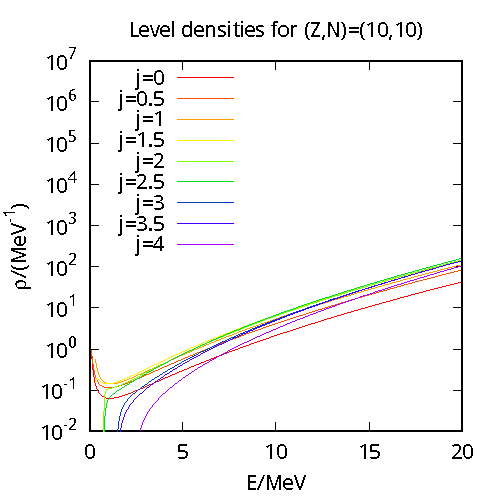
\includegraphics[width=\bredd\textwidth]{figures/rho/Z10N10.pdf}\label{sfig:rhoj:a}}
&
\subfloat[Without compensating for the yrast energy.]{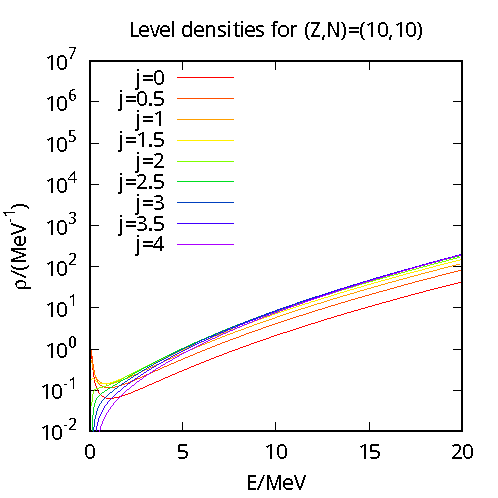
\includegraphics[width=\bredd\textwidth]{figures/rho/Z10N10_no-yrast.pdf}\label{sfig:rhoj:b}}
\end{tabular}
\caption{\label{fig:rhospin} The energy dependence of the level density of $~^{20}\mathrm{Ne}$ for spin $J=0,\tfrac{1}{2},\dots, 4$. In order to be able to compare level densities for different spin at the same effective energy above the yrast line, the yrast energy has not been subtracted from $E_\text{eff}$ in \ref{sfig:rhoj:b}.}
\end{center}
\end{figure}

%In order to get a picture of how all of this comes together, we plot the level density for the $A=10$ isobar for $J=0, \tfrac{1}{2}, \dots, 4$. 
The level density of $~^{20}\mathrm{Ne}$ for different spin with and without subtracting the yrast-energy is illustrated in \autoref{fig:rhospin}. 
As can be seen in the figure, the level densities for higher spin start at a lower value for low energies, way lower than $\unit[1]{level/MeV}$, which indicates that the continous view of energy levels fails at these energies. 
The spins appear to be split up in $2$ groups, one for $J \le 1$ and one for $J>1$.
The level densities for $4 \ge J> 1$ initially grow rapidly, until they overtake the lower spin level densities and settle at a seemingly proportional relationship with each other. As a result of the $(2J+1)\exp{(-(J+1/2)^2)}$ dependence on $J$, moderate $J$ values give the largest level density.
The same general behaviour is seen for the other nuclei at the $A=20$ isobar.

In order to see if this is a general feature of our model, we also investigate $~^{99}\mathrm{Zr}$ -- this nucleus is being chosen arbitrarily as an example of a non-fissile nucleus far form the $A=20$ isobar. The corresponding plots of the level densities are seen in \autoref{fig:rhospin2}. We note that the inclusion of the yrast energy is not nearly as significant for the spins under consideration, since the larger value of $\Theta$ reduces the yrast energy of a given $J$. This also explains why $J=4$ has the highest density of states in this case: a higher $\Theta$ means that the $\exp{(-(J+1/2)^2/\Theta)}$ factor does not supress the level density as rapidly with increasing spin. 
We also see that it is only for $J\ge 3$ that we see the hint of a dip for lower energies. This could perhaps indicate that the pronounced spin-dependence seen for the $A=20$ isobar will reveal itself for yet higher spin -- a natural consequence of the higher moment of inertia for heavier nuclei.

\begin{figure}
\begin{center}
\begin{tabular}{cc}
\subfloat[The level densities derived from \eqref{eq:rho}.]{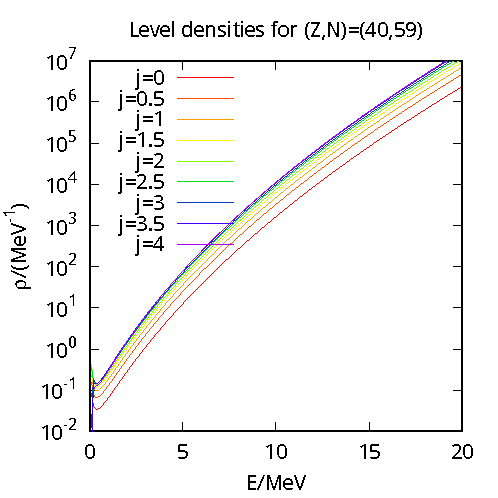
\includegraphics[width=\bredd\textwidth]{figures/rho/Z40N59.pdf}\label{sfig:rhoj2:a}}
&
\subfloat[Without compensating for the yrast energy.]{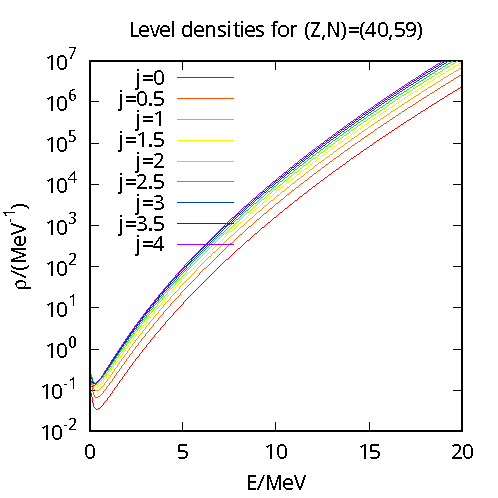
\includegraphics[width=\bredd\textwidth]{figures/rho/Z40N59_no-yrast.pdf}\label{sfig:rhoj2:b}}
\end{tabular}
\caption{\label{fig:rhospin2} The energy dependence of the level density of $~^{99}\mathrm{Zr}$ for spin $J=0,\tfrac{1}{2},\dots, 4$. In order to be able to compare level densities for different spin at the same effective energy above the yrast line, the yrast energy has not been subtracted from $E_\text{eff}$ in \ref{sfig:rhoj2:b}.}
\end{center}
\end{figure}

In any case, this is low-energy behaviour, and both the Fermi gas model\cite{grossjean1985} and the very notion of a continuous level density has problems for low energies. Most notably, the Fermi gas model itself, without compensating for shell and pairing effects, predicts a singularity at $U=0$, which is why we see an increase in the level density for lower energies and spin in both \autoref{fig:rhospin2} and in \autoref{fig:rhospin}, which have been truncated at $E=\unit[0.1]{MeV}$ in order to avoid this.

The level density was also investigated for a fixed spin for different isotopes of the $A=20$ isobar, but no conclusive trends were found.

On the other hand, for the isotope $Z=10$, the level density for higher energies generally increases with additional neutrons, which is to be expected, since there are more ways to arrange the nucleons for a given excitation energy, this is illustrated in \autoref{fig:Z10-rho}, where the brighter lines correspond to heavier nuclei.

\begin{figure}
\begin{center}
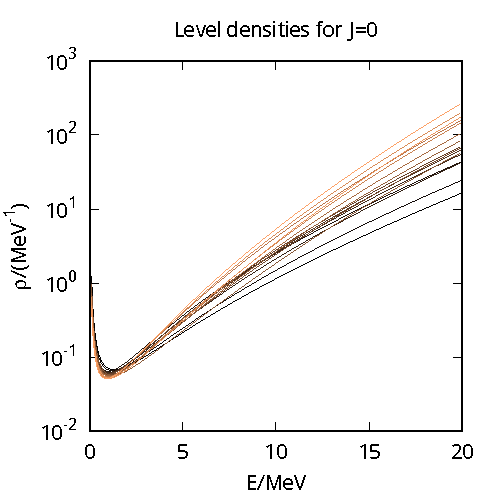
\includegraphics[width=0.6\textwidth]{figures/rho/Z10_N7-N22.pdf}
\caption{\label{fig:Z10-rho} The level densities for $~^{17}\mathrm{Mg}$ to $~^{32}\mathrm{Mg}$, where brigther lines correspond to heavier nuclei.}
\end{center}
\end{figure}

\clearpage
\subsubsection{Transition Probabilities}
The decay width $\Gamma_{\nu,l}$ into a given final energy interval $[E_f,E_f+dE]$ by particle $\nu$ with orbital angular orbital momentum $l$ also depends on the transition probability $T_l(\epsilon_\nu)$.

One of the more well-known models of a transition probability by particle decay is the Gamow model for alpha decay, in which the mother nucleus $(Z,N)$ is modeled as essentially being composed of a ``ready-to-go'' alpha particle and the daughter nucleus $(Z-2,N-2)$ and the probability to decay is given by the probability for the alpha particle to tunnel through the potential due to the daughter nucleus, with an additional factor depending on how often the alpha particle has a chance to tunnel. 

This model is readily generalized to other particle decays: we may just as well imagine a proton being formed inside the mother nucleus $(Z,N)$, and tunneling through the potential from the daughter nucleus $(Z-1,N)$.

In order to make this model quantitative, we need an actual potential. Approximating the charge distribution of the daughter and tunneling particle as spherical, we may model the potential due to electrostatic interaction as a simple Coulomb potential, which gives us
\begin{equation}
V = V_\text{Col} + \dots =  Z_1 Z_2 \frac{e^2}{r_{12}} + \dots,
\end{equation}
in non-rationalized units.
If we go ahead and assume that not only the charge distribution, but the potential as a whole is spherically symmetric, we can employ the standard procedure of separating the problem into a radial and angular part, where the radial potential is given by
\begin{equation}
V_\text{r} = Z_1 Z_2 \frac{e^2}{r_{12}} + \frac{l(l+1)\hbar^2}{2\mu r^2} + \dots\quad .
\end{equation}
Here we still need additional terms to take the effective nucleon-nucleon intraction into account. The assumption of spherical symmetry also gives us the angular part of the wave function as a spherical harmonic, determing the angular distribution of the emitted particle in the center-of-mass frame.

\begin{figure}
\begin{center}
\input{figures/pot-theory/proximity.pdf_t}
\caption{\label{fig:prox} A schematic sketch of how the proximity approximation is carried out. Two close surfaces are approximated as a series of parallel surfaces, which in turn are approximated as infinite parallel surfaces, for which the potential energy is easier to calculate. This result is then summed up for all parallel surfaces.}
\end{center}
\end{figure}

The nuclear part of the potential used by \prgname{Codex} is a proximity potential\cite{gollerthan:1988:thesis}\cite{blocki1977}. 
Proximity potentials may be derived from a more general approximation method, in which two nearby surfaces are divided into several parallel surfaces, close enough to be approximated as semi-infinite, see \autoref{fig:prox}\cite{fosco:2012}. The contributions from the different sets of parallel surfaces are assumed to be additive.
The potential energy is calculated for these slabs, and factors to correct for the actual geometry are introduced. This approach is widely used in Casimir force calculations between objects of a more arbitrary shape\cite{fosco:2011}. This approximation is also known by ``Derjaguin approximation'' in other fields\cite{fosco:2012}.

In the nuclear case, the situation is somewhat complicated by the fact that the form of the nucleon-nucleon interaction is unknown. As such, there exist several proximity potentials\cite{dutt:2010}. Dutt et. al. showed that 12 common proximity potentials were able to predict fusion barrier heights within $10\%$ of the experimental values for asymmetric fusion reactions ranging from $~^{12}\mathrm{C} + ~^{17}\mathrm{O}$ to $~^{86}\mathrm{Kr} + ~^{208}\mathrm{Pb}$\cite{dutt:2010}. Proximity-type potentials have also been used to study alpha and proton decay\cite{proton-alpha-proxy:2005}\cite{proton-proxy:2010}, which is closer to our intended application\footnote{It is not immediately obvious to the author if the assumptions of the proximity potential formalism applies to proton or alpha decay. It does however reproduce experimental half-lives to a reasonable degree, see e.g. Balasubramaniam and Arunachala\cite{proton-alpha-proxy:2005}, this is for emission from heavier nuclei, though.}.

The proximity potential is given by
\begin{equation}
V_\text{N} = C \phi(\zeta),\label{eq:vn}
\end{equation}
where $\phi(\zeta)$ is the so-called \emph{universal function}, which for a given nucleon-nucleon interaction is independent of the geometry of the nuclei in the proximity approximation. $\zeta$ is a unitless distance between the two nuclei, see below. Geometrical factors are contained in the proportionality ``constant'' $C$, which is given by
\begin{equation}
C = 4\pi \gamma b \frac{r_{c,1} r_{c,2}}{r_{c,1} + r_{c,2}}
\end{equation}
where $\gamma$ is the surface energy coefficient, which can be approximated by
\begin{equation}
\gamma= 0.9517 (1.0 - 1.78260 \times I^2),
\end{equation}
where $I=(N-Z)/A$ is the neutron excess.

We use the universal function by Blocki, 1997,
\begin{equation}
\phi(\zeta)= \begin{cases}-0.5(\zeta-2.54)^2-0.0852(\zeta-2.54)^3 & \zeta < 1.2511 \\
-3.437\exp{(-\zeta/0.75)} & \zeta > 1.2511,\qquad\cite{blocki1977}
\end{cases}\label{eq:prox}
\end{equation}
where $\zeta$ is the distance between the two nuclear surfaces, normalized with respect to the typical surface diffuseness $b$ of the nuclei, here taken to be $\unit[1]{fm}$\cite{blocki1977}. More explicitly, we have
\begin{equation}
\zeta = \frac{r - r_\text{sum}}{b},
\end{equation}
where $b$ is the surface diffuseness, and $r_\text{sum}$ is roughly the sum of the radii of the two nuclei, so that $r-r_\text{sum}$ gives the distance between the nuclear surfaces\cite{blocki1977}. An effective sharp nuclear surface may be estimated by the formula
\begin{equation}
r_\text{sharp} = 1.28 A^{1/3} - 0.76 + 0.8 A^{-1/3}\quad\unit{fm}.\qquad\cite{blocki1977}\label{eq:sharp}
\end{equation}
%which in \prgname{CODEX} is adjusted by adding a radius correction constant, $r_\text{adj} = \unit[0.9]{fm}$.
\autoref{eq:sharp} is used to estimate the radii of all nuclei, and as a result $r_\text{sharp}=\unit[1.32]{fm}$ for protons and neutrons, which is slightly different from the value of $r_0$ that is normaly used.
%!!!  THE INPUT FILE SAYS ``VAZ ET. AL.'' NEXT TO RADIUS CORRECTION. WHAT IS THIS? !!!
In the proximity potential, it is preferable to use the \emph{central radius} $r_\text{c}$ rather than the effective sharp radius\cite{blocki1977}, which is given by 
\begin{equation}
r_\text{c} =r_\text{sharp} \left(1-\left(\tfrac{b}{r_\text{sharp}}\right)^2\right)\quad.\qquad\cite{myers1973}
\end{equation}
Hence, $r_\text{sum} = r_\text{c,1}+r_\text{c,2}$. 

%!!!THIS WILL BE MORE CLEAR ONCE I WRITE SOMETHING GENERAL ABOUT THE MODEL, WHICH REALLY DEALS WITH BULK AND SURFACE ENERGIES OF A THIN-SKINNED SYSTEM.!!!

Since the proximity model takes the spatial extent of the nuclei into account, we modify the Coloumb-interaction accordingly, from that of a point particle to that of a homogenously charged, solid sphere
\begin{equation}
V_\text{C} = \begin{cases}\frac{Z_1 Z_2 e^2}{r} &\quad r>r_\text{ch} \\ \frac{Z_1 Z_2 e^2}{r_\text{ch}^2}(3-(r/r_\text{ch})^2) &\quad r<r_\text{ch}, \end{cases}
\end{equation}
where we here use the more common formula for the charge radius, $r_\text{ch} = r_0 A^{1/3}$.

 In \autoref{fig:np-Z10N10}, we illustrate the total potential of $~^{20}\mathrm{Ne}$ for tunneling of protons and neutrons. The individual contributions to the total potential may be discerned by looking at the potential for the emission of $l=0$ neutrons (which are only affected by the proximity potential) and $l=0$ protons (which have to tunnel through the sum of the Coulomb and the proximity potential). %Since these potentials are only used for tunneling calculations, their shape below $E=0$ is not significant, since the particles cannot escape if their energy is less than $0$, and we will hence not display the $V<0$ parts in subsequent figures, in order to focus on the relevant details.
On this energy scale, the barrier the protons have to tunnel through is merely \unit[2]{MeV} high, but since the proton separation energy for $~^{20}\mathrm{Ne}$ is \unit[12]{MeV}, it will only happen for excitation above \unit[12]{MeV}, as the proton does not have a positive energy otherwise. Neutrons with a positive energy and $l=0$ do not have to tunnel at all, and exist as resonances above the potential barrier. The tunneling formalism does not apply in this case, and we instead use \eqref{eq:t0n}, which we discuss later.

We also see that the centrifugal part quickly dominates, essentially a result of protons and neutrons being relatively light particles: for $\alpha$-decay, the centrifugal part is about a fourth of the values displayed above, and the $l$-dependence of the tunneling probability is not very significant for low $l$\cite{weisskopf:1979}.  
This strong $l$-dependence makes proton radioactivity a sensitive probe for the orbital angular momentum of valence protons for proton emitting nuclei\cite{proton-alpha-proxy:2005}. However, in this case, it also poses a problem, since, for high $l$-values, it removes the potential well created by the Coulomb and proximity potential. Even for moderate $l$ values, it makes particles with low energy classically forbidden within the the radius of barrier (see \autoref{fig:np-Z10N10}), which appears inconsistent with the picture of a preformed particle tunneling through said barrier.
The solution adopted in this work is to assign probability zero to tunnel for particles that are classically forbidden within the nucleus. This will supress decay for higher $l$, since the bottom of the potential well rises as $l$ does. For a higher $l$, the potential well disappears entirely\footnote{Another solution, attractive since we do not use the potential to estimate separation energies, is to model the strong interaction as an infinitely deep potential that cancels the centrifugal part, so that bound particles can always exist in the nucleus. The common $V=-\infty$ for $r<r_\text{nucleus}$ potential achieves this. Another solutions found in the literature is to have other, finite potentials below certain radii, but -- in non-relativistic quantum mechanics -- this goes against the assumption of spherical symmetry unless the effective nucleon-nucleon interaction depends on $l$ so to exactly cancel the centrifugal part.}.

\begin{figure}
\begin{center}
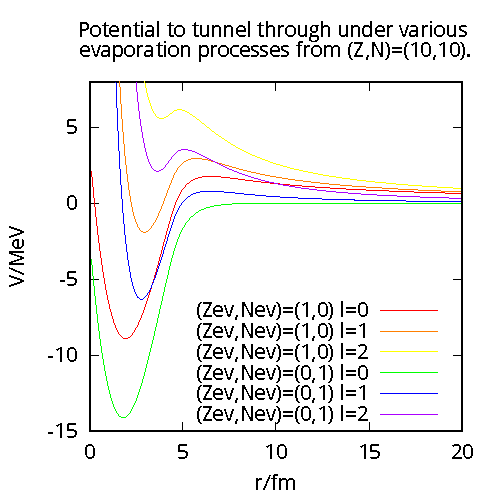
\includegraphics{figures/pot/np-potZ10N10.pdf}
\caption{\label{fig:np-Z10N10} The potential used for tunneling of neutrons and protons with $l=0,1,2$ from $~^{20}\mathrm{Ne}$. The potential for $l=0$ neutrons is exactly the proximity potential \eqref{eq:prox}, while the $l=0$ proton's potential show the sum of the proximity and Coulomb potential. }
\end{center}
\end{figure}

Given the potential, the transition probability can be calculated in the WKB approximation as 
\begin{equation}
T_l(\epsilon_\nu) = \exp{(-2G)},\qquad\cite{krane:book}
\end{equation}
where 
\begin{equation}
G=\sqrt{\frac{2\hbar}{\mu}} \int_{r_1}^{r_2} \sqrt{V_l(r)-\epsilon_{\nu}}\,dr.
\end{equation}
The classical turning points, $r_1$ and $r_2$, are the inner and outer radii for which the kinetic energy is equal to the potential energy. It should be noted that the WKB approximation is not, strictly speaking, valid for regions where the potential is approximately constant over several wave-lengths $\lambda=\frac{2\pi}{k}$, which will not be valid for at the turning points, since $\lambda \to \infty$. 
A somewhat more refined WKB approximation formula is
\begin{equation}
T_l(\epsilon_\nu) = \frac{1}{1+\exp{2G}},\qquad\cite{kemble}
\end{equation}
 which still suffers from the same short-comings as the previous formula. Nevertheless, the transition amplitudes calculated with the WKB formula are generally of the right order of magnitude, which should suffice for our purposes\cite{2011arXiv1106.1065N}.

For $\epsilon>V_\text{max}$, we can no longer view the emission as tunneling, because the particle passes ``over'' the barrier. Instead, we use
\begin{equation}
T_l = \frac{1}{1+\exp{\left(-\frac{2\pi}{\hbar \omega}(E-V_\text{max}))\right)}},\label{eq:tlabove}
\end{equation}
where
\begin{equation}
\hbar\omega = \hbar\sqrt{\frac{1}{\mu}\left(\frac{d^2V_l}{dr^2}\right)_{r_\text{max}}}.\qquad\cite{gollerthan:1988:thesis}
\end{equation}
We use yet another formula for $l=0$ neutrons, which do not have a barrier to tunnel through, and for which \autoref{eq:tlabove} cannot be applied, since no maximum exists. Instead, we use the transmission coefficient for transmission over a step 
\begin{equation}
T_{0,\text{n}} = \frac{4\sqrt{E}\sqrt{E+V_0}}{(\sqrt{E}+\sqrt{E+V_0})^2},\label{eq:t0n}
\end{equation}
where we use the depth $V_0=\unit[40]{MeV}$, the value being chosen to approximate the depth of the nuclear potential\cite{welldepth}. This was the formula used in \prgname{Codex}.

The transmission coefficients corresponding to the potentials in \autoref{fig:np-Z10N10} are presented in \autoref{fig:np-tZ10N10}.  We see that the $l=0$ neutrons do not behave as expected, in that they have a lower transmission coeffiecient than both protons and $l=1$ neutrons. We also see the very sudden increase of the transmission coeffiecients for higher $l$-values, a result of our choice to set the transmission probability to zero for $E<V_{l,\text{min}}$ and to not cut the centrifugal potential below some $r$-value.

\begin{figure}
\begin{center}
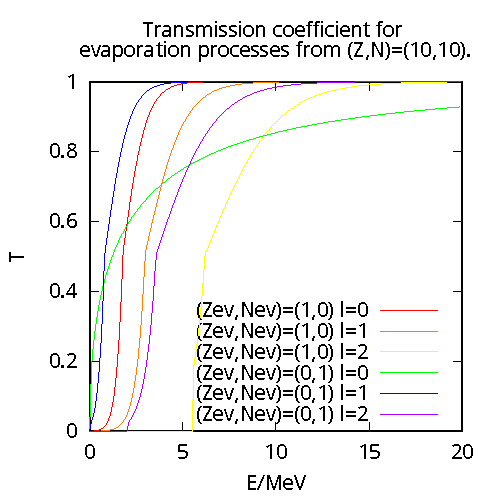
\includegraphics{figures/pot/np-transZ10N10.pdf}
\caption{\label{fig:np-tZ10N10} The transmission coefficients for evaporation of neutrons and protons with $l=0, 1, 2$; from $~^{20}\mathrm{Ne}$. }
\end{center}
\end{figure}

\paragraph{$\gamma$-decay}
The above discription concerns the tunneling of a nucleon or cluster through a potential barrier, and is thus not applicable to $\gamma$-decay.

Gamma transition rates are usually expressed in terms of a strength function, $f_{Xl}$, like
\begin{equation}
T_l(E) = E^{2l+1} f_{Xl}(E).\label{eq:gammat}
\end{equation}
The factor $E^{2l+1}$ factorizes out the energy dependence from semi-classical radiation theory, so that the strength function contains the nuclear information. $X$ here refers to the type of radiation, electric or magnetic.

There are many ways in which a nucleus can emit photons, and hence several kinds of strength functions.  For our purposes, collective excitations are the most important, and the modes that dominate are the \emph{Giant resonance}, in particular the $E1$, $E2$ and $M1$ modes\cite{ripl:2006}. These collective excitations are vibrational in nature, and give rise to Lorentzian strength functions.

%Since our model does not implement parity, the $E1$ will dominate over the $M1$, and we thus use an $E1$ strength function for all $l=1$ $\gamma$-radiation. %!!! IS THIS TRUE FOR COLLECTIVE EX? !!!
The strength functions used in this work are
\begin{equation}
\begin{aligned}
T_{E1} =  \frac{ZN}{A}\frac{4e^2}{3\pi u\hbar} \frac{E_\gamma \Gamma_{E1}}{(E_\gamma^2 -E^2_0)^2+(E_\gamma \Gamma_{E1})^2}  \\
T_{E2} =  \frac{6Z e^2}{25\pi\hbar^3 u}R^2\left(1+\frac{5}{2}\frac{b^2}{R^2}\right)  \sum_j \frac{1}{2}\frac{E_\gamma \Gamma_{E2}}{(E_{\gamma}^2 -E^2_{0j})^2+(E_\gamma \Gamma_{E1})^2},
\end{aligned}
\end{equation}
where $R=r_0 A^{1/3}$ is the nuclear radius and $b$ the surface diffuseness, a parameter also used in the proximity potential. The presence of $Z$ and $N$ in the above equations are to account for the number of nucleons participating in the excitation\cite{Chomaz:1997}.
The peak values are given by
\begin{equation}
\begin{aligned}
E_{0,E1} = \frac{80}{A^{1/3}}\unit{MeV}, &\\
E_{01,E2} = \frac{63}{A^{1/3}}\unit{MeV} &\frac{130}{A^{1/3}}\unit{MeV}.
\end{aligned}
\end{equation}
The value $80/A^{1/3}$ is supposedly a good fit for medium to heavy weight nuclei\cite{Chomaz:1997}, while the $63/A^{1/3}$ and $130/A^{1/3}$ are too diffuse to reliably observe in light nuclei\cite{PhysRevLett.34.748}\cite{speth1991electric}. As such, it may be desirable to use other values for light nuclei, as well as adding in the possibility of an $M1$-transition.





%Instead, $\gamma$-ray \emph{strength functions} $f_{Xl}$ can be used to calculate transition probabilities by $\gamma$-ray emission, 
%\begin{equation}
%T_l(E) = E^{2l+1} f_{Xl}(E),\label{eq:gammat}
%\end{equation}
%where $f_{XL}$ in principle can depend on whether the transition is electric or magnetic, $X=E$ or $X=M$, respectively. In fact, \eqref{eq:gammat} can almost be viewed as a definition of the strength function. 
%A more precise definition of the strength function between states $i$ and $f$ is:
%\begin{equation}
%f_{ifXl}^J = \frac{\Gamma_{\langle i\rangle fXl}}{E^{2l+1}_\gamma}\rho_{J}(E_i),\qquad\cite{ainp:1973}
%\end{equation}
%where $\langle i\rangle $ signifies that $\Gamma_{\langle i\rangle fXl}$ is averaged over states (with fixed $J$) in a region around the initial state. This definition is reasonable in the context of sufficiently excited nuclei decaying to, for example, the ground state, since the small spacing of the levels around the initial state does not allow them to be experimentally distinguished, and hence the measured decay width will be the sum of the decay widths of all those states, $\Gamma_\text{exp} = \sum_{i \in [E,E+\Delta E]} \Gamma_{ifXl}$. The average quantity$ \Gamma_{\langle i\rangle fXl}$ may than be formed by dividing with the total number of states in this region, $\rho_J(E_i) \Delta E$, and from this we get that
%\begin{equation}
%f_{ifXl}^J = \frac{\sum_{i \in [E,E+\Delta E]} \Gamma_{ifXl}}{\Delta E} \frac{1}{E^{2l+1}_\gamma} = \frac{\Gamma_\text{exp}}{\Delta E} \frac{1}{E^{2l+1}_\gamma},
%\end{equation}
%which would be an alternative definition. The factor $E^{2l+1}$ is a matter of definition: it factorizes out the $l$-dependence from semi-classical radiation theory.
%The difference between our decay width, given by \eqref{eq:gammagamma}, and the expression above is that we also have a smeared out final state, and to get the total probability to decay to any of them, we multiply the above $\Gamma$ by $\rho(E^*_f)$.
%
%Of course, our definition above does nothing to specify the shape of the strength function, unless we already know $\Gamma_{ifXl}$.  
%
%The transmission coefficient used by \prgname{CODEX} ... !!!TODO!!!
